\chapter{Evaluation}

\section{Results}

To determine how well the cSVD implementation performs, three tests are conducted. The first test measures computation time, the second test measures the Mean Squared Error (MSE) of the estimated singular values, and the third test measures the reconstruction error w.r.t. of EDJMs. For the computation time test PyTorch is used, but otherwise MATLAB is used. The reason is MATLAB is easier to create graphs with, and the algorithm does not change significant behavior whether Python or MATLAB is used.

\subsection*{Computation Time}

To test the computation time the \texttt{time} library in Python is used. On Linux this library is able to provide microsecond resolution. Algorithm \ref{alg:result:performance} shows pseudocode of how the test is conducted. This code tests the computation time of PyTorch SVD and the four different cSVD implementations. In the pseudocode \texttt{svdAlgorithm} refers to the PyTorch SVD and the cSVD implementations. The test procedure measures the computation time for each \texttt{svdAlgorithm} 10 times, on a new random tensor of $25 \times 10000 \times 784$, generated as in \eqref{eq:csvd:rand}, every iteration. The reason a random tensor is used instead of an actual EDJM is because the performance does not change based on the input data being sparse or not. The cSVD implementations are configured to compute the 10\% largest singular values, with an oversampling value $p=20$ because that is the realistic use case of the cSVD algorithm when calculating the score.

\begin{equation}
  \label{eq:csvd:rand}
  X \sim \mathcal{N}_{25 \times 10000 \times 784}(0, 1)
\end{equation}

$ $ \newline

\begin{algorithm}[H]
\label{alg:result:performance}
\For{$i \gets 1$ \KwTo $10$}{
  $X \gets \mathrm{rand}(25, 10000, 784)\mathrm{.to}(\mathrm{GPU})$ \\
  $\mathrm{synchronizeCUDA}()$ \\
  $\mathrm{svdStartTime} \gets \mathrm{currentTimeMicroSec}()$ \\
  $U,S,V \gets \mathrm{svdAlgorithm}(X)$ \\
  $\mathrm{synchronizeCUDA}()$ \\
  $\mathrm{svdEndTime} \gets \mathrm{currentTimeMicroSec}()$ \\
  $\mathrm{svdTime}[i] \gets \mathrm{svdEndTime} - \mathrm{svdStartTime}$
}
\KwResult{csvdTime}
\caption{Performance test procedure}
\end{algorithm}

$ $ \newline

To reduce the data of the 10 trials for each \texttt{svdAlgorithm} the mean and variance are computed to make them comparable.The mean and variance are computed as \eqref{eq:result:mean} and \eqref{eq:result:var}.

\begin{equation}
  \label{eq:result:mean}
  \hat \mu = \frac{1}{10} \sum_{i=1}^{10} \mathrm{csvdTime}_i 
\end{equation}

\begin{equation}
  \label{eq:result:var}
  \hat \sigma^2 = \frac{1}{10} \sum_{i=1}^{10} \left ( \mathrm{csvdTime}_i - \hat \mu \right )^2
\end{equation}

Table \ref{tab:csvd:performance} shows the results for the PyTorch SVD compared with the four cSVD implementations. The speedup shows how many times larger the mean computation time of the PyTorch SVD is compared to the cSVD implementations.

\begin{table}[H]
  \centering
    \begin{tabular}{|l|l|l|l|l|} \hline
      Implementation & $\hat \mu$ & $\hat \sigma^2$ & Speedup & Speedup per EDJM \\ \hline
      PyTorch SVD & 10.172 & 0.0082 & * & * \\ \hline
      Sequential cSVD & 1.0961  & 53.085e-03 & 9.280 & 9.280 \\ \hline
      Partially sequential cSVD & 1.095 & 97.853e-03 & 9.294 & 9.294 \\ \hline
      Batch cSVD & 0.034 & 2.872e-06 & 301.741 & 11.967 \\ \hline
      Batch cSVD (\texttt{gesvda}) & 0.037  & 0.149e-06 & 274.240 & 10.997 \\ \hline
    \end{tabular}
    \caption{Mean computation time, variance and speedup over 10 trials.}
    \label{tab:csvd:performance}
\end{table}

\subsection*{Mean Square Error}

For the MSE test the four feed-forward DNN configurations in Table \ref{tab:dnn:score} are used. Rather than training them for the same accuracy, they are trained over 20 epochs. The reason is that the accuracy of the DNNs are not important, the only necessary feature is the EDJMs are sparse. Figure \ref{fig:csvd:mse} shows the MSE of the singular values of the EDJMs, using a cSVD implementation in MATLAB. The MSE of the EDJMs are calculated as in \eqref{eq:csvd:mse}. The error term $\hat \sigma_i - \sigma_i$ is normalized with $\sigma_i$ as a large error term isn't necessarily large compared to the actual singular value. 

\begin{equation}
  \label{eq:csvd:mse}
    MSE = \frac{1}{k} \sum_{i=1}^{k} \left ( \frac{\hat \sigma_i - \sigma_i}{\sigma_i} \right )^2
\end{equation}
  
\begin{figure}[H]
  \centering
  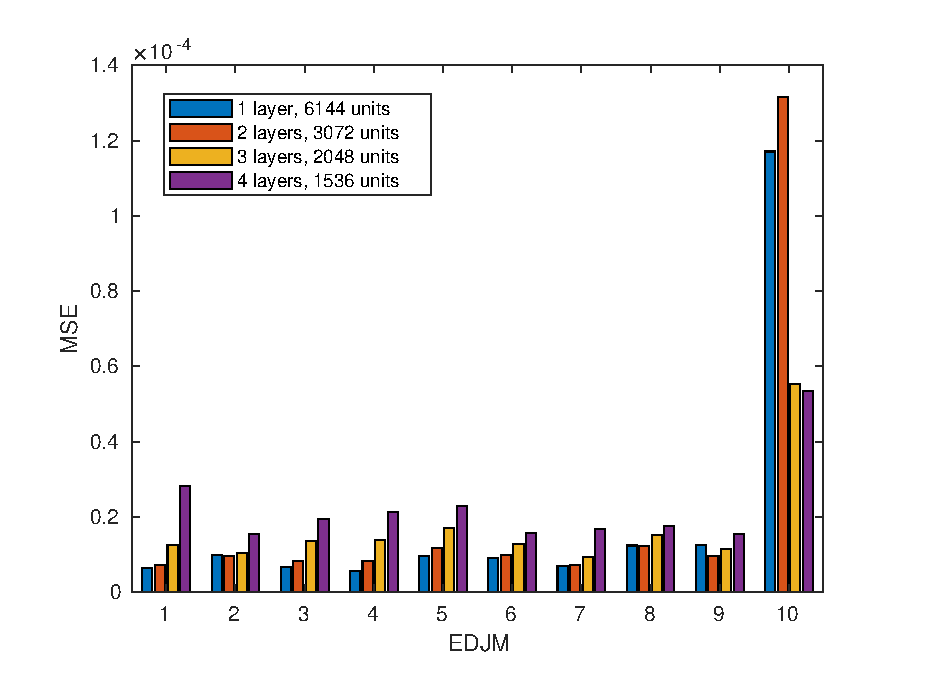
\includegraphics[scale=0.6]{Figures/csvd_mse.eps}
  \caption{cSVD MSE with $k=78$ and oversampling $p=20$.}
  \label{fig:csvd:mse}
\end{figure}

\subsection*{Reconstruction Error}

The reconstruction error test is conducted on the same 40 EDJMs as the MSE test, using both cSVD and full SVD implementations in MATLAB. The reconstruction error determines how close a rank-k approximation $X_k$ is to the input EDJM $X$. The rank-k approximation is shown in \eqref{eq:recon:svd}.

\begin{equation}
  \label{eq:recon:svd}
  \begin{split}
    U,S,V &= \mathrm{svdAlgorithm}(X) \\
    X_k &= USV^T
  \end{split}
\end{equation}

Erichson, et. al. uses \eqref{eq:csvd:recon} \cite{erichson:csvd} to compute the reconstruction error. As with the MSE, the reconstruction error also normalizes the error. The reason is that a large error isn't necessarily large compared to the correct value.

\begin{equation}
  \label{eq:csvd:recon}
  \mathrm{reconstruction\ error} = ||X - X_k^T||_F/||X||_F = ||X - USV^T||_F/||X||_F
\end{equation}

Figure \ref{fig:csvd:reconstruction} shows the reconstruction using the MATLAB cSVD implementation and Figure \ref{fig:svd:reconstruction} shows the reconstruction using MATLAB's SVD.

\begin{figure}[H]
  \centering
  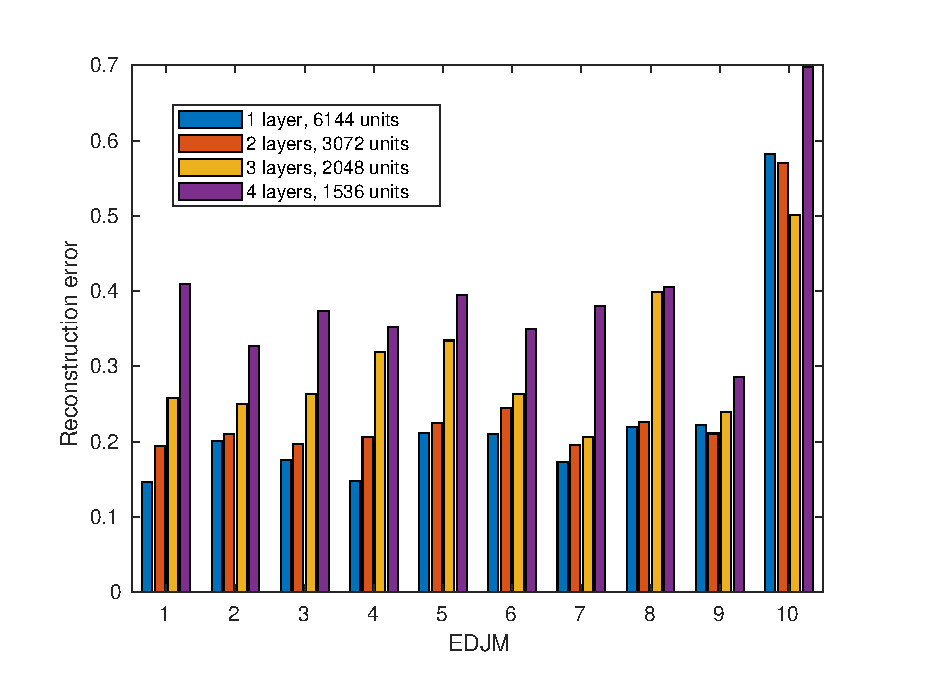
\includegraphics[scale=0.6]{Figures/csvd_reconstruction.eps}
  \caption{cSVD reconstruction with $k=78$ and oversampling of $p=20$.}
  \label{fig:csvd:reconstruction}
\end{figure}

\begin{figure}[H]
  \centering
  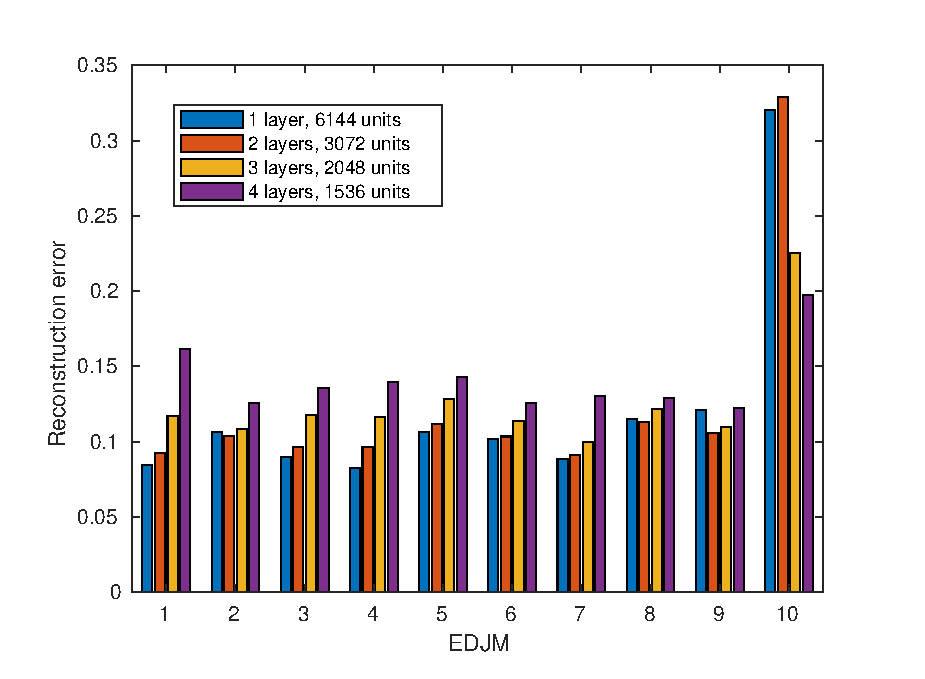
\includegraphics[scale=0.6]{Figures/svd_reconstruction.eps}
  \caption{SVD reconstruction with $k=78$.}
  \label{fig:svd:reconstruction}
\end{figure}

\newpage

\section{Discussion}

% what did the results show
% do the results make sense
% are the results good
% why did gesvda perform worse

The computation time test shows the cSVD using the 10\% largest singular values do not result in a 10\% speedup. A part of this is because there is an oversampling of 20, which means more intermediate singular values are computed than the end result. In this case there are 98 intermediate singular values which is 20 more than the final 78, which contributes to the performance gap. Comparing the sequential and partially sequential implementation reveals how small a factor the batch multiplication plays compared to the eigenvalue decomposition and SVD. The importance of these two are highlighted by the performance increase between the sequential and batched cSVD. The performance in the batched cSVD beats the sequential cSVD, even per EDJM. This shows that cuSOLVER can beat MAGMA at these matrix sizes and more benchmarking has to be done to determine when they perform best. The reason for why the cSVD using \texttt{gesvda} performed worse than without it unknown, more testing has to be conducted to determine if \texttt{gesvda} is better at larger batch sizes than the batche eigenvalue decomposition.

Even though the speedup using the cSVD algorithm is very good, it is also important that the approximated singular values are close to the actual singular values. The MSE test shows this is the case, with the MSE being neglible. This also confirms the EDJMs are indeed sparse when using the ReLU activation functions. If the cSVD were to be used to calculate the score for DNNs using activation functions other than ReLU, there would have to be conducted benchmarks to determine if they introduce enough sparsity for the cSVD to work. Although the cSVD is able to compute the 10\% largest singular values with a very small error, the low-rank approximation of the EDJMs in the reconstruction test shows the orthonormal matrices are not approximated well. This reveals the EDJMs, although sparse, are not sparse enough to be approximated with 10\% largest singular values. There has to be conducted more tests to determine how the oversampling and singular value threshold has an effect on the reconstruction error.

One method that may be able to improve the reconstruction error is to determine if there is some structure in EDJMs based on training data, because this can be used to create a basis transform $\Psi$ for the EDJMs. Using a basis transform will have an up front performance cost as it requires a matrix multiplication, but it may be possible to get a better reconstruction error with less singular value threshold or oversampling.

\newpage

\section{Conclusion}

This project began with trying to answer \textit{How can singular value decomposition be parallelized?} This was divided into three subquestions with a specific focus on the score problem.

\subsubsection*{Which algorithms can be used to compute an SVD in parallel?}

There are multiple algorithms to compute the SVD in parallel, but most compute all of the singular values which is not necessary to compute the score. The solution is to use the Compressed Singular Value Decomposition (cSVD). This algorithm can compute the largest singular values set by a threshold, which in the case of computing score should be the 10\% largest singular values. The algorithm works by assuming the input matrix is sparse, which means it can reduce computation problem by taking random samples of the input matrix.

\subsubsection*{How can the the time complexity w.r.t. amount of data ($N$), data input size ($d_{in}$) and data output size ($d_{out}$) be reduced?}

By using the cSVD algorithm, the time complexity w.r.t. the data input size becomes smaller because of the random sampling. When calculating singular values of an EDJM the computational problem grows by $0.1d_{in}^2$ rather than $d_{in}^2$, because it is only necessary to calculate the 10\% largest singular values (10\% translates to a factor of 0.1).

cSVD does not solve the problem of reducing the complexity w.r.t. the amount of data or the output size. But it is possible to decrease the computation time as the output size grows, as output size means more EDJMs to compute the SVD for. The solution is to compute each individual SVD in parallel as they do not depend on each other.

\subsubsection*{Which type of computing platform is suitable for implementation?}

The cSVD algorithm is well suited to implement on GPUs because all but two steps of the algorithm are easy to parallelize. These two steps require an eigenvalue decomposition, which is possible to do on both CPU and GPU. By using a pure GPU implementation of the eigenvalue decomposition it is possible to make a scalable cSVD implementation. This allows applying SVD on many EDJMs simultaneously. This type of problem is suited for high-performance computing platforms using multiple GPUs in clusters.